\documentclass{report}

\usepackage[utf8]{inputenc}

\usepackage{float}
\usepackage{graphicx}
\usepackage{caption}
\usepackage{subcaption}
\usepackage{amsfonts}
\usepackage[dvipsnames]{xcolor}

\usepackage{svg}
\usepackage{amsmath}
\usepackage{amsthm}
\usepackage{amssymb}
\usepackage{mathabx}

\usepackage{ulem}

\usepackage{cancel}

\usepackage{listings}
\usepackage{hyperref}
\hypersetup{
    colorlinks=true,
    allcolors=blue,
    }

\usepackage{geometry}
 \geometry{
 a4paper,
 left=15mm,
 top=20mm,
 right = 15mm,
 bottom = 20mm
 }

\usepackage{fancyhdr}
\setlength{\headheight}{15.2pt}
\pagestyle{fancy}
\fancyhead[RO]{\chaptermark}
\fancyfoot{}
\fancyfoot[R]{Page \thepage}

\usepackage[style=authoryear-ibid,backend=biber]{biblatex}
\addbibresource{bibliography.bib}

\theoremstyle{definition}
\newtheorem{definition}{Definition}[section]
\newtheorem{example}{Example}[section]
\newtheorem{exercise}{Exercise}[section]
\newtheorem{proposition}{Proposition}[section]
\newtheorem{theorem}{Theorem}[section]
\newtheorem{lemma}{Lemma}[section]
\newtheorem{axiom}{Axiom}
\newtheorem{corollary}{Corollary}[section]
\theoremstyle{remark}
\newtheorem{remark}{Remark}[section]
\newtheorem{question}{Question}[section]
\newtheorem{answer}{Answer}[section]

\usepackage{subfiles}

\usepackage{changepage}

\usepackage{framed}

\newcommand{\AND}{\wedge}
\newcommand{\OR}{\vee}
\newcommand{\NOT}{\neg}
\newcommand{\EMPTY}{\varnothing}

\newcommand{\UNDER}{\uline}

\newcommand{\newpar}{\vspace{\baselineskip}\par\noindent}

\title{Point Cloud to Sectional Area Curve}
\author{Stamatis Stamatelopoulos}

\begin{document}

\maketitle
 
\tableofcontents

\chapter{Testing}

\section{\texttt{test-1.cpp}}\label{sec:test-1}

\newpar The so-called {\it extended Wigley Hull form} \parencite{journee1992experiments} has a 
simple analytic formulation which permits the exact calculation
of it's cross-sectional area curve. We use this example to test 
the accuracy of \texttt{SectionalAreaXwiseYsymmetrical()} to verify. While the standard
Wigley hull is a rather poor geometry, in the extended version, 
by varying the parameters $c_1,\ c_2$ and $c_3$ outside their
prescribed domains $[0,1]$ richer geometries can be generated
even if they no longer represent a hull-form. The one used here is 
retrieved from the sample space by setting $L = 2$, $B=0.5$, $T = 0.2$, 
$c_1 = 5.2$, $c_2 = 2.1$ and $c_3 = 2.3$ (see Figure \ref{fig:test-1-wigley-render}).
\begin{figure}[H]
    \centering
    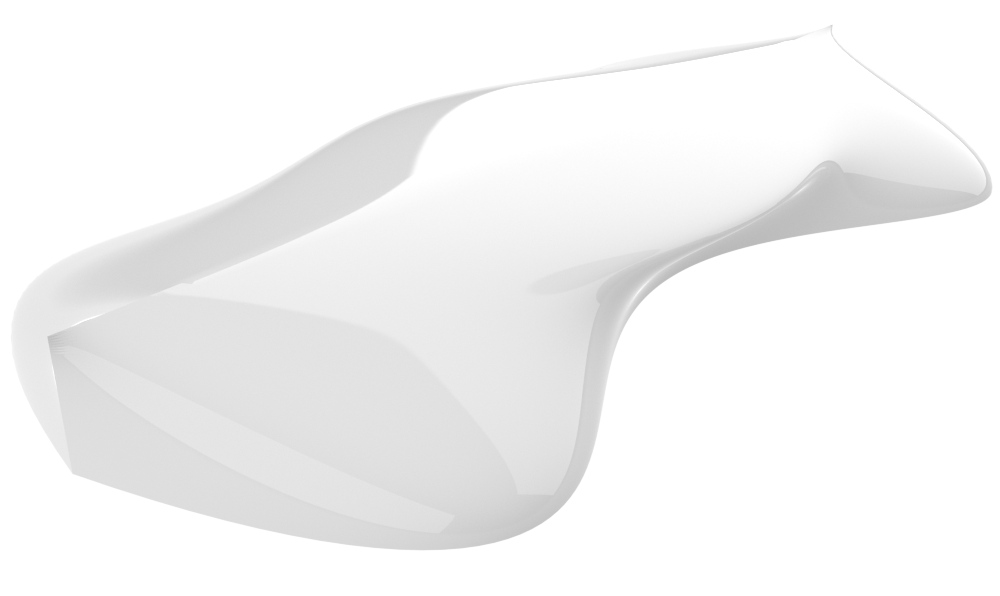
\includegraphics[width=1.0\linewidth]{figures/test-1-wigley-render.png}
    \caption{Geometry used in \texttt{test-1.cpp}. $L = 2$, $B=0.5$, $T = 0.2$, 
    $c_1 = 5.2$, $c_2 = 2.1$ and $c_3 = 2.3$}
    \label{fig:test-1-wigley-render}
\end{figure}

\newpar The \texttt{SectionalAreaXwiseYsymmetrical()} procedure works with 
a point cloud as input, in order to calculate the cross sectional areas, {\it along the 
X-direction}, of the underlying geometry. Naturally, said geometry must comply 
with certain assumptions: given a solid bounded by a surface,
\begin{enumerate}
    \item It must be symmetrical with respect to the XZ plane passing through the origin
    and the point cloud must all lie on one side of it (either positive Y or negative Y)
    \item It does not have to be convex, however it must be star-convex with respect to 
    the XZ plane: for every point $p = (p_1,p_2,p_3)$ on the bounding surface, the line between
    $(p_1,0,p_3)$ and $p$ must be completely contained in the solid
    \item The point cloud provided must be entirely on the boundary surface (i.e. not on the 
    solid whose boundary is the given surface)
\end{enumerate}
The point cloud provided will directly affect the accuracy of the result, in the sense that uniform point 
clouds might perform better than arbitrarily generated ones. Nevertheless, for this 
experiment, the point clouds generated are randomly sampled from the 
boundary surface's domain. 
\newpar Now, the scheme employed in \texttt{SectionalAreaXwiseYsymmetrical()} has the following
seven steps
\begin{enumerate}
    \item Identify the domain of the sectional area curve, parametrized in accordance with 
    the actual surface coordinates
    \item Discretize the identified domain in $N$ sub-domains $[a_i,b_i]\ i=1,...,N$, each referring to a specific
    section. Specifically, given the domain $[a,b]$, $N\in\mathbb{N}$ and $\lambda\in\mathbb{R}$, first generate 
    $t_i = a + (b-a)(i-1)/(N-1)$ for $i=1,...,N$. Then, set $a_0 = a$, $b_N = b$, $l = (t_1-t_0)\lambda$  and $a_i = t_{i-1} - \lambda$,
    $b_i = t_i + \lambda$ for all other $i$.
    \item Group the point cloud in terms of this discretization, assigning every point $p=(p_1,p_2,p_3)$, to the sub-domain 
    $[a_i,b_i]$ where $a_i \le p_2 < b_i$, thereby generating $N$ such groupings
    \item For every grouping, project all points on the plane $(a_i/2+b_i/2, u, v)$ along $(1,0,0)$
    \item For every grouping, sort points Z-wise
    \item For every grouping sum up the rectangles formed by consecutive points $p, q$ by the following 
    four vertices: $(pq),\ (p\tilde{p}),\ (q\tilde{q})$ and $(\tilde{p}\tilde{q})$, where for $x=(x_1,x_2,x_3)$,
    $\tilde{x}=(x_1,0,x_3)$
    \item For every grouping multiply the total resulting area by $2$
\end{enumerate}
\newpar We proceed by a brief investigation of the effect of the following parameters, on the 
accuracy of the approximation: (1) size of the generated point cloud (2) number of points 
to evaluate the sectional area at (3) $\lambda\in[0,1]$ to determine for each sectional area,
how many neighboring points are considered. From the relevant experimentation, it seems that 
the determination of this parameters is an information issue: the more information (large point cloud),
the more sectional-area curve points can be requested with sufficient accuracy, which is to be expected.
However, this means that depending on the application (i.e. calculation of sectional area curve derivatives 
via finite differences), a relatively small point cloud might be sufficient. We begin with the generation of 
a point cloud in 3000 points, each randomly sampled from the surface's domain (see Figures \ref{fig:test-1-wigley-render-3K-point-cloud-1} and \ref{fig:test-1-wigley-render-3K-point-cloud-2}).
\begin{figure}[H]
    \centering
    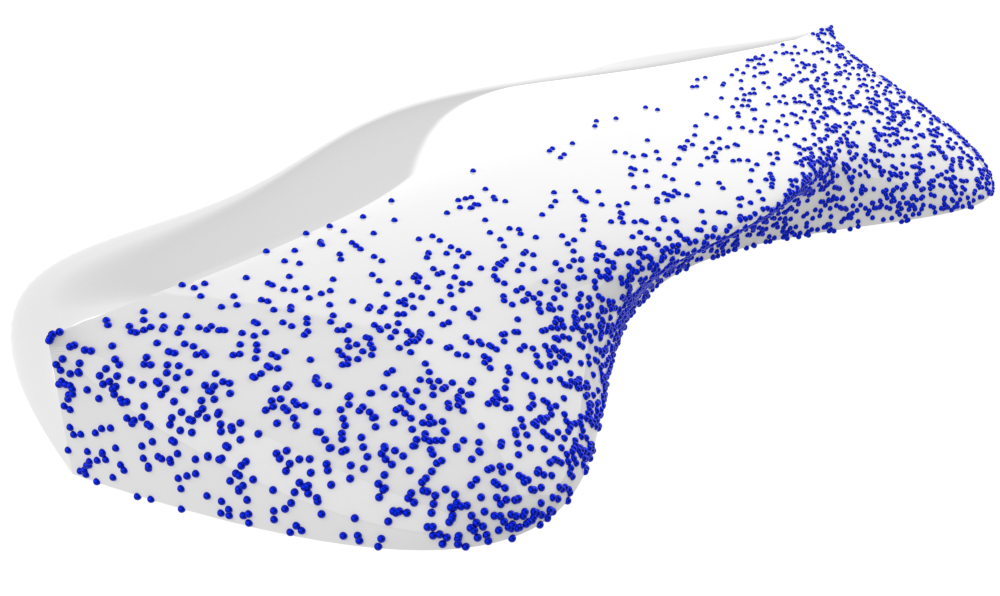
\includegraphics[width=1.0\linewidth]{figures/test-1-wigley-render-3K-point-cloud-1.png}
    \caption{3000 points randomly generated on the surface, top view}
    \label{fig:test-1-wigley-render-3K-point-cloud-1}
\end{figure}
\begin{figure}[H]
    \centering
    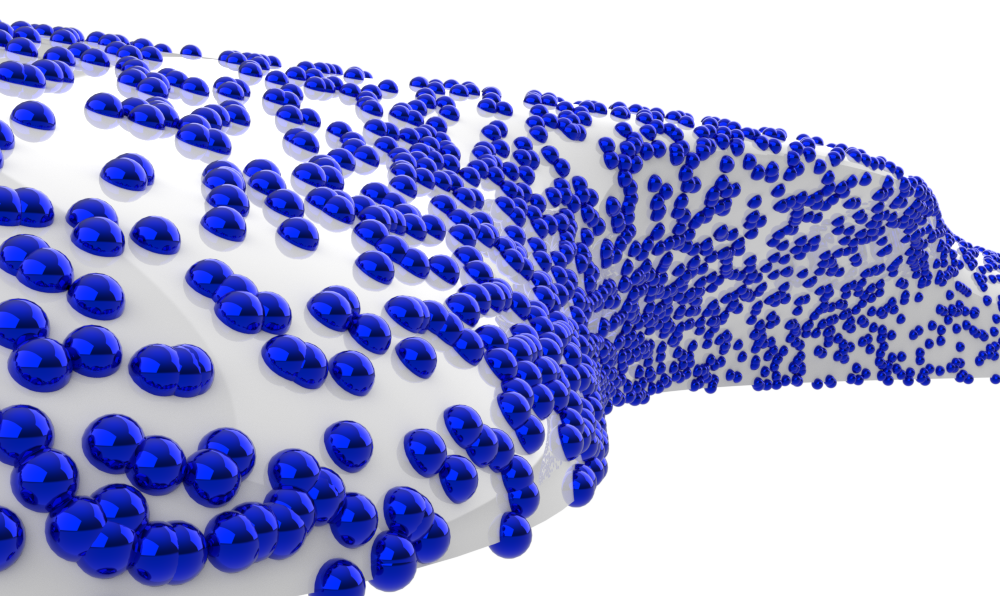
\includegraphics[width=0.7\linewidth]{figures/test-1-wigley-render-3K-point-cloud-2.png}
    \caption{3000 points randomly generated on the surface, bottom view}
    \label{fig:test-1-wigley-render-3K-point-cloud-2}
\end{figure}
\newpar Then, let $N=10$ and $\lambda = 1.0$, so that all the points in the point cloud are used. Looking in Figure \ref{fig:test-1-sac-3K-l-100-N-10}, this selection
of $N$, $\lambda$ results in an $L^\infty$ error of $0.00711$ at the calculated points. Part of this error is caused by using points 
far away from the longitudinal point of evaluation to evaluate the sectional area curve. If we instead limit the this selection by setting 
$\lambda = 0.78$, the error can be reduced to $0.00332$ (see Figure \ref{fig:test-1-sac-3K-l-78-N-10}).
\begin{figure}[H]
    \centering
    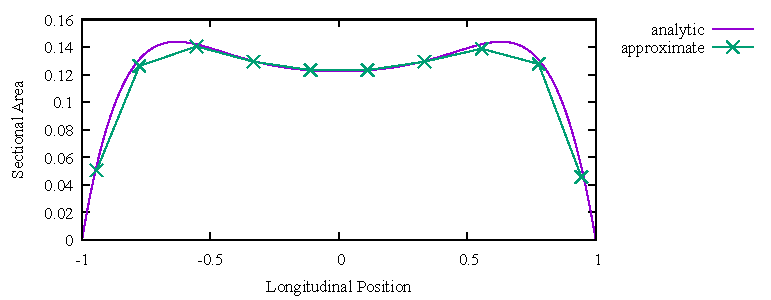
\includegraphics[width=0.7\linewidth]{figures/test-1-sac-3K-l-100-N-10.pdf}
    \caption{Sectional area curve at $N=10$ points, of the geometry depicted in Figure \ref{fig:test-1-wigley-render},
    using 3000 randomly sampled points, and $\lambda = 1.0$. The $L^\infty$ error at the evaluated points is $0.00711$}
    \label{fig:test-1-sac-3K-l-100-N-10}
\end{figure}
\begin{figure}[H]
    \centering
    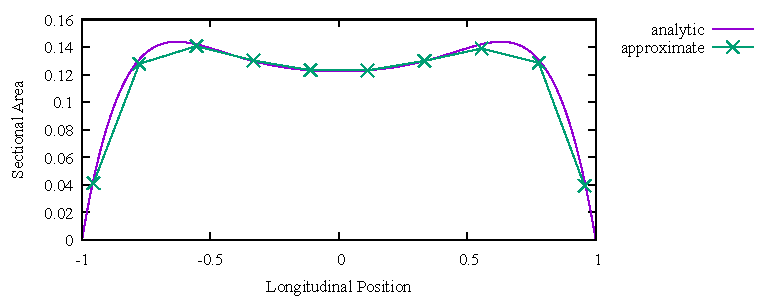
\includegraphics[width=0.7\linewidth]{figures/test-1-sac-3K-l-78-N-10.pdf}
    \caption{Sectional area curve at $N=10$ points, of the geometry depicted in Figure \ref{fig:test-1-wigley-render},
    using 3000 randomly sampled points, and $\lambda = 0.78$. The $L^\infty$ error at the evaluated points is $0.00332$}
    \label{fig:test-1-sac-3K-l-78-N-10}
\end{figure}
\newpar Finally, Figures \ref{fig:test-1-wigley-render-3K-l-78-N-10-1} and \ref{fig:test-1-wigley-render-3K-l-78-N-10-2} illustrate
this selection, where the bronze cubes are the points that were used to calculate each cross section's area.
\begin{figure}[H]
    \centering
    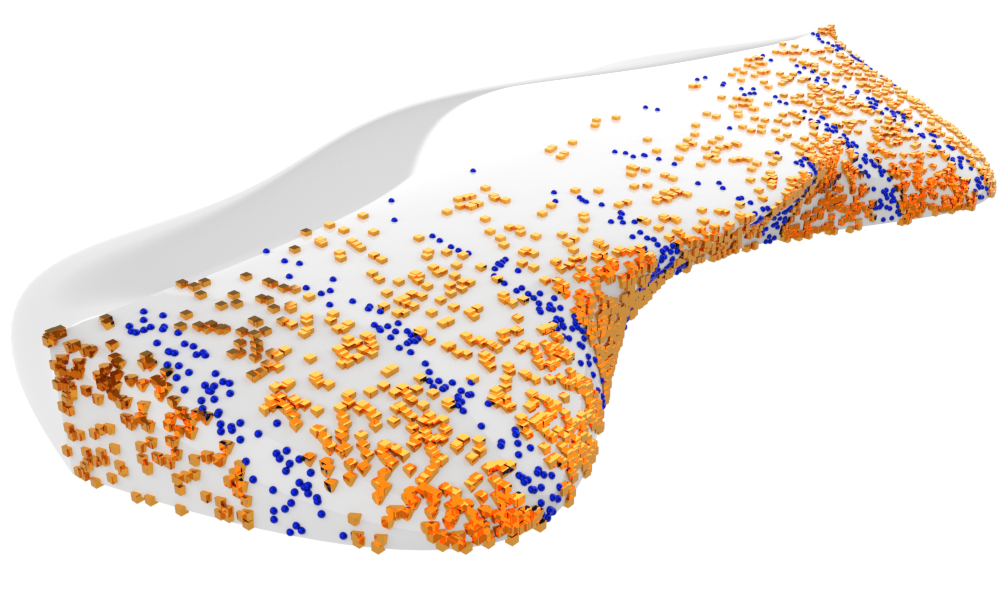
\includegraphics[width=1.0\linewidth]{figures/test-1-wigley-render-3K-l-78-N-10-1.png}
    \caption{3000 points randomly generated on the surface. The bronze cubes depict the sub-selection
    of on-surface points when $N=10$ and $\lambda = 0.78$. Top view}
    \label{fig:test-1-wigley-render-3K-l-78-N-10-1}
\end{figure}
\begin{figure}[H]
    \centering
    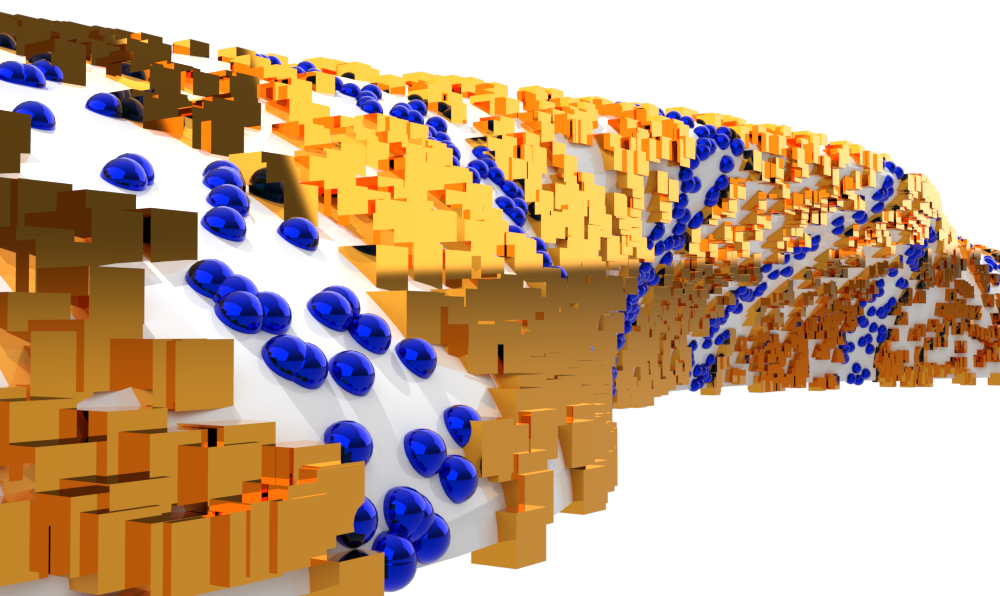
\includegraphics[width=0.7\linewidth]{figures/test-1-wigley-render-3K-l-78-N-10-2.png}
    \caption{3000 points randomly generated on the surface. The bronze cubes depict the sub-selection
    of on-surface points when $N=10$ and $\lambda = 0.78$. Bottom view}
    \label{fig:test-1-wigley-render-3K-l-78-N-10-2}
\end{figure}
\newpar Continuing to reduce $\lambda$ does not further increase performance as there is 
not enough information (point cloud size) to do so, which clarifies the balance between 
deviation due to insufficient amount of information and deviation due to too much information (using 
points further far away from the point where the sectional area is evaluated at). See Figure \ref{fig:test-1-sac-3K-l-20-N-10} for the
resulting sectional area curve with error $0.00642$ if $\lambda=0.2$ and Figure \ref{fig:test-1-wigley-render-3K-l-20-N-10-1} for the on-surface selection.
\begin{figure}[H]
    \centering
    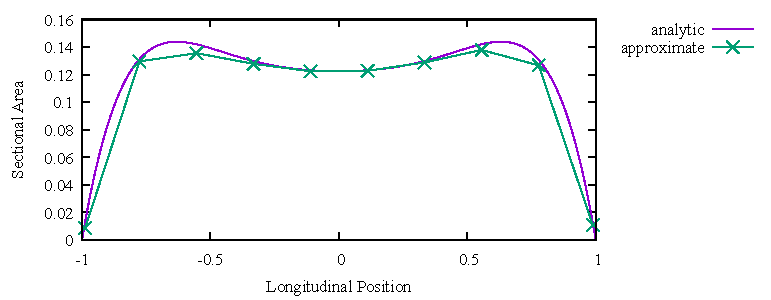
\includegraphics[width=0.7\linewidth]{figures/test-1-sac-3K-l-20-N-10.pdf}
    \caption{Sectional area curve at $N=10$ points, of the geometry depicted in Figure \ref{fig:test-1-wigley-render},
    using 3000 randomly sampled points, and $\lambda = 0.2$. The $L^\infty$ error at the evaluated points is $0.00642$}
    \label{fig:test-1-sac-3K-l-20-N-10}
\end{figure}
\begin{figure}[H]
    \centering
    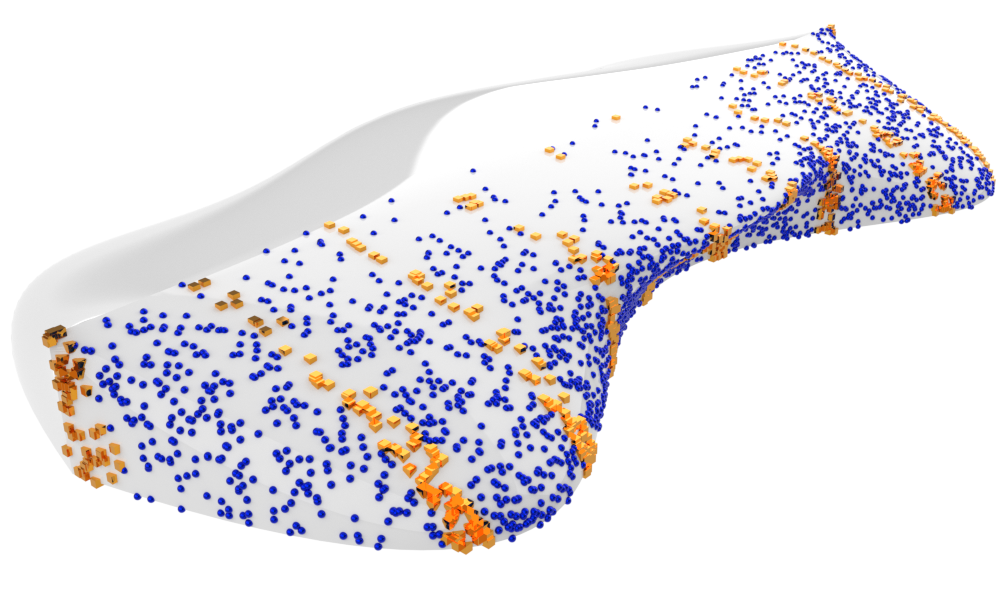
\includegraphics[width=1.0\linewidth]{figures/test-1-wigley-render-3K-l-20-N-10-1.png}
    \caption{3000 points randomly generated on the surface. The bronze cubes depict the sub-selection
    of on-surface points when $N=10$ and $\lambda = 0.2$. Top view}
    \label{fig:test-1-wigley-render-3K-l-20-N-10-1}
\end{figure}

\section{\texttt{test-2.cpp}}

\newpar \texttt{SectionalAreaXwiseYsymmetrical()} can be used to numerically evaluate the derivatives of the sectional area curve.
For example, generating 1000 points to the aft and to the bow the extended wigley hull (see Section \ref{sec:test-1}), then evaluating 
the cross sectional area at five points and using the first two calculate the 1-point finite-difference derivative, an accuracy of 
0.001 relative to the analytic derivative is achieved (see Figure \ref{fig:test-2-1K-l-100-derivatives})
\begin{figure}[H]
    \centering
    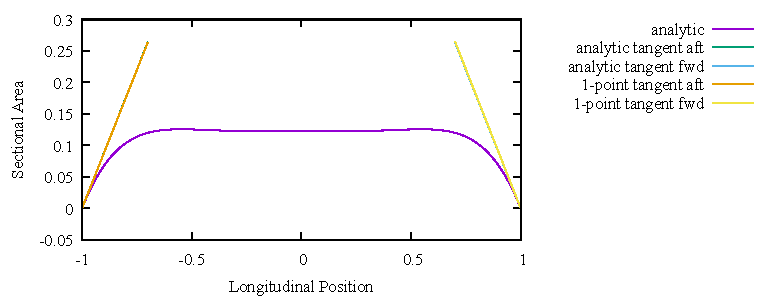
\includegraphics[width=0.7\linewidth]{figures/test-2-1K-l-100-derivatives.pdf}
    \caption{1st derivatives of sectional area curve evaluated through 1-point finite differences using \texttt{SectionalAreaXwiseYsymmetrical()}. 
    1000 points were generated at aft and bow. The relative difference between the approximate
    and analytic derivatives is in the order of 0.001}
    \label{fig:test-2-1K-l-100-derivatives}
\end{figure}

\section{\texttt{test-3.cpp}}\label{sec:test-3}

\newpar The cross sectional area curve of the KCSsim hull (see \texttt{KCSsim.hpp} modeller and \cite{KHAN2022103339}) is calculated 
using \texttt{SectionalAreaXwiseYsymmetrical()} routine. Since the analytic sectional area curve of 
the KCSsim hull is not available, the validity of the produced curve is verified through it's 
integral which must be equal to the volume of the underlying geometry. Said integral is approximated 
numerically, while the volume is calculated through a triangulation of the KCSsim hull in 5e4 triangles.

\begin{figure}[H]
    \centering
    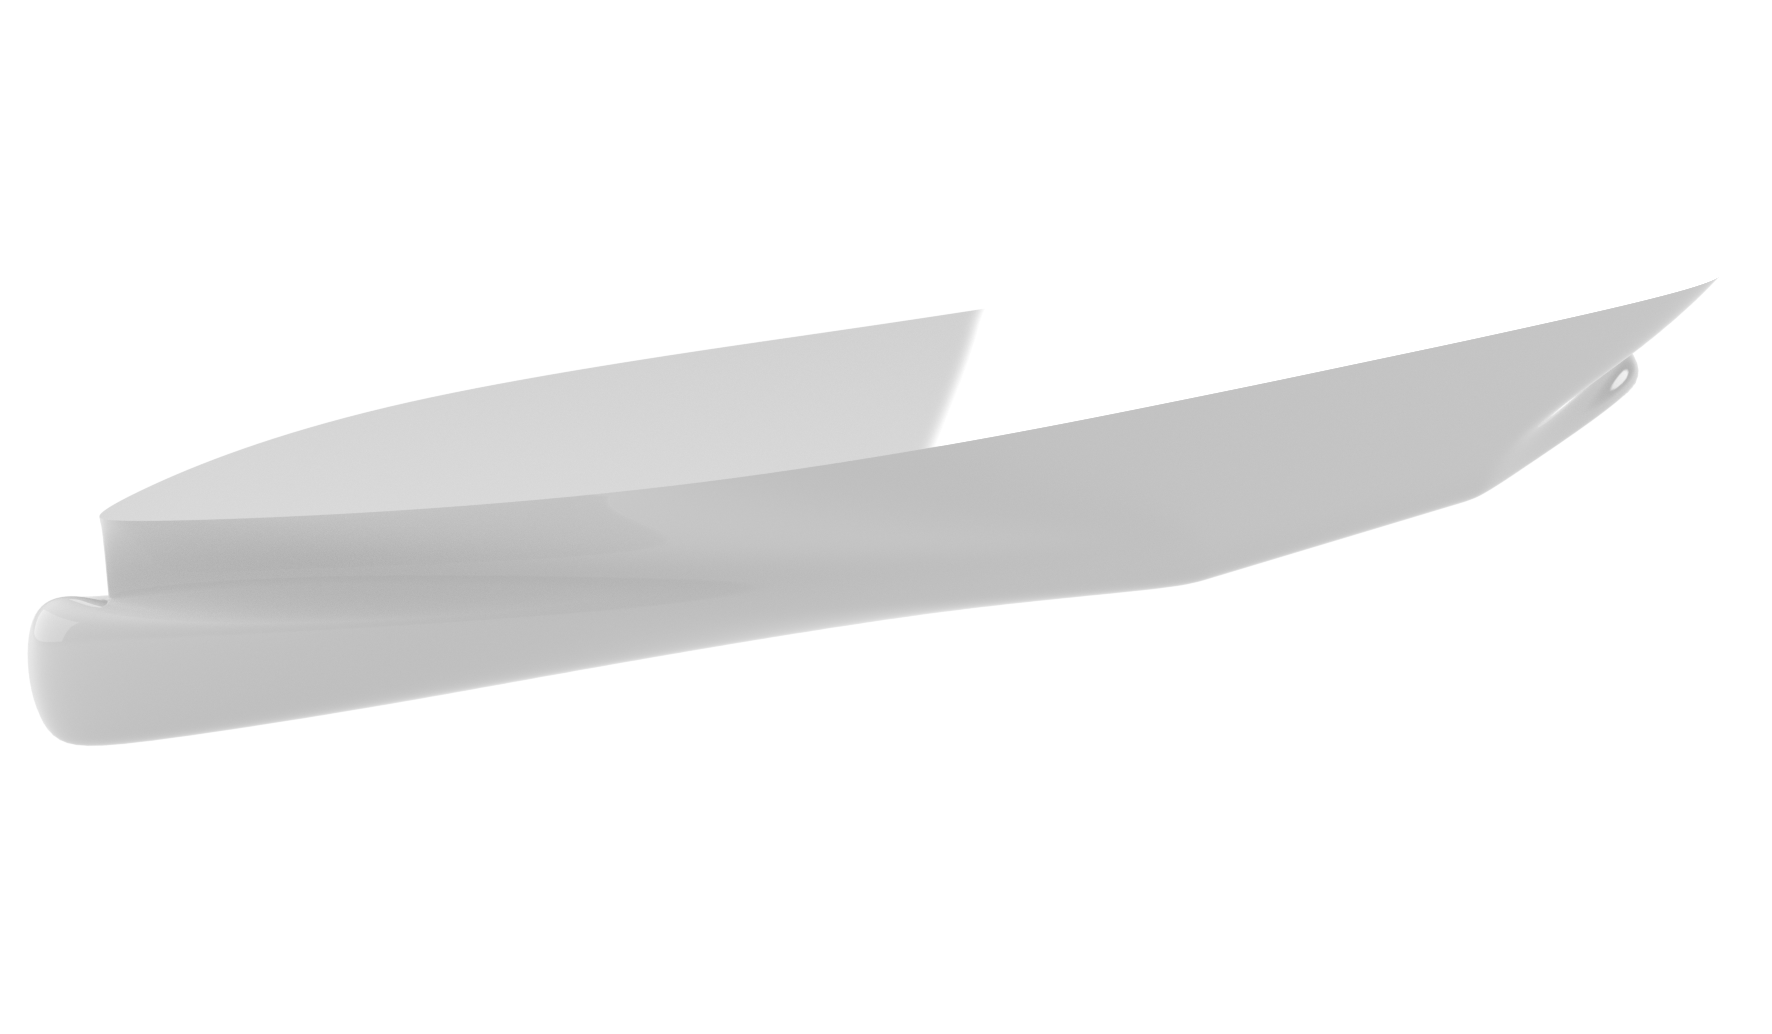
\includegraphics[width=\linewidth]{figures/test-3-kcssim-render.png}
    \caption{Rendered KCSsim hull. Design is documented in Table \ref{tab:test-3-kcssim-design}}
    \label{fig:test-3-kcssim-render}
\end{figure}
\begin{table}[H]
    \centering
    \begin{tabular}{|c|c|c|c|c|c|}
        \hline 
        Parameter & Value & Parameter & Value & Parameter & Value\\
        \hline 
        $c_1$ & 1.0 & $c_{11}$ & 0.5 & $c_{21}$ & 1.0 \\
        \hline 
        $c_2$ & 0.8 & $c_{12}$ & 0.5 & $c_{22}$ & 0.0\\
        \hline 
        $c_3$ & 0.8 & $c_{13}$ & 0.5 & $c_{23}$ & 0.5 \\
        \hline 
        $c_4$ & 0.265 & $c_{14}$ & 0.5 & $c_{24}$ & 0.5 \\
        \hline 
        $c_5$ & 0.543 & $c_{15}$ & 0.5 & $c_{25}$ & 0.5 \\
        \hline 
        $c_6$ & 0.0 & $c_{16}$ & 0.05 & $c_{26}$ & 0.5 \\
        \hline 
        $c_7$ & 0.3 & $c_{17}$ & 0.5 & $c_{27}$ & 0.5 \\
        \hline 
        $c_8$ & 0.65 & $c_{18}$ & 0.7 & $c_{28}$ & 0.5 \\
        \hline 
        $c_9$ & 0.7 & $c_{19}$ & 0.8 & $c_{29}$ & 0.5 \\
        \hline 
        $c_{10}$ & 0.5 & $c_{20}$ & 1.0 & - & - \\
        \hline 
    \end{tabular}
    \caption{Design parameters of KCSsim hull rendered in Figure \ref{fig:test-3-kcssim-render}}
    \label{tab:test-3-kcssim-design}
\end{table}
\newpar Now, two points clouds have been generated, one random and one uniform, both having 3e4 points and 
the resulting sectional area curves are depicted in Figure \ref{fig:test-3-sac-random-uniform}. 
\begin{figure}[H]
    \centering
    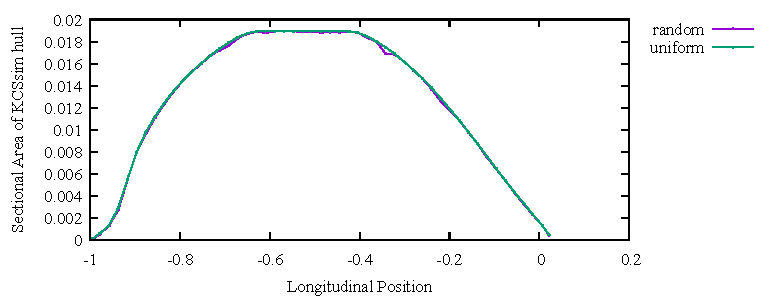
\includegraphics[width=0.7\linewidth]{figures/test-3-sac-random-uniform.pdf}
    \caption{Sectional area curves from 51 sections, evaluated for the KCSsim hull documented 
    in Table \ref{tab:test-3-kcssim-design}, using a random and a uniform point cloud in 3e4
    points and $\lambda = 1.0$ in \texttt{SectionalAreaXwiseYsymmetrical()}. Even though the uniform
    sectional area curve is smoother that it's random counterpart, integrating them in order to 
    derive the volume of the underlying geometry, yields a smaller error for the random-case. Specifically,
    the relative errors compared to the actual volume, for the uniformly and randomly generated 
    point clouds were 0.01188 and 0.00564 respectively.}
    \label{fig:test-3-sac-random-uniform}
\end{figure}
\newpar As is noted in Figure \ref{fig:test-3-sac-random-uniform}, the randomly-generated point 
cloud outperformed the uniformly generated one. The reason is that the uniformly generated point cloud was restricted to the iso-curves of the surface, thereby
leaving large areas of the geometry empty, which was not the case with the randomly-generated one.
This is illustrated in Figures \ref{fig:test-3-kcssim-random-uniform-render} and 
\ref{fig:test-3-kcssim-random-uniform-render-close-up}, where the uniform point cloud (blue spheres),
identify the contours of the surface's iso-curves, while the randomly-generated point cloud, covers the surface 
more evenly (ironically, more uniformly).

\begin{figure}[H]
    \centering
    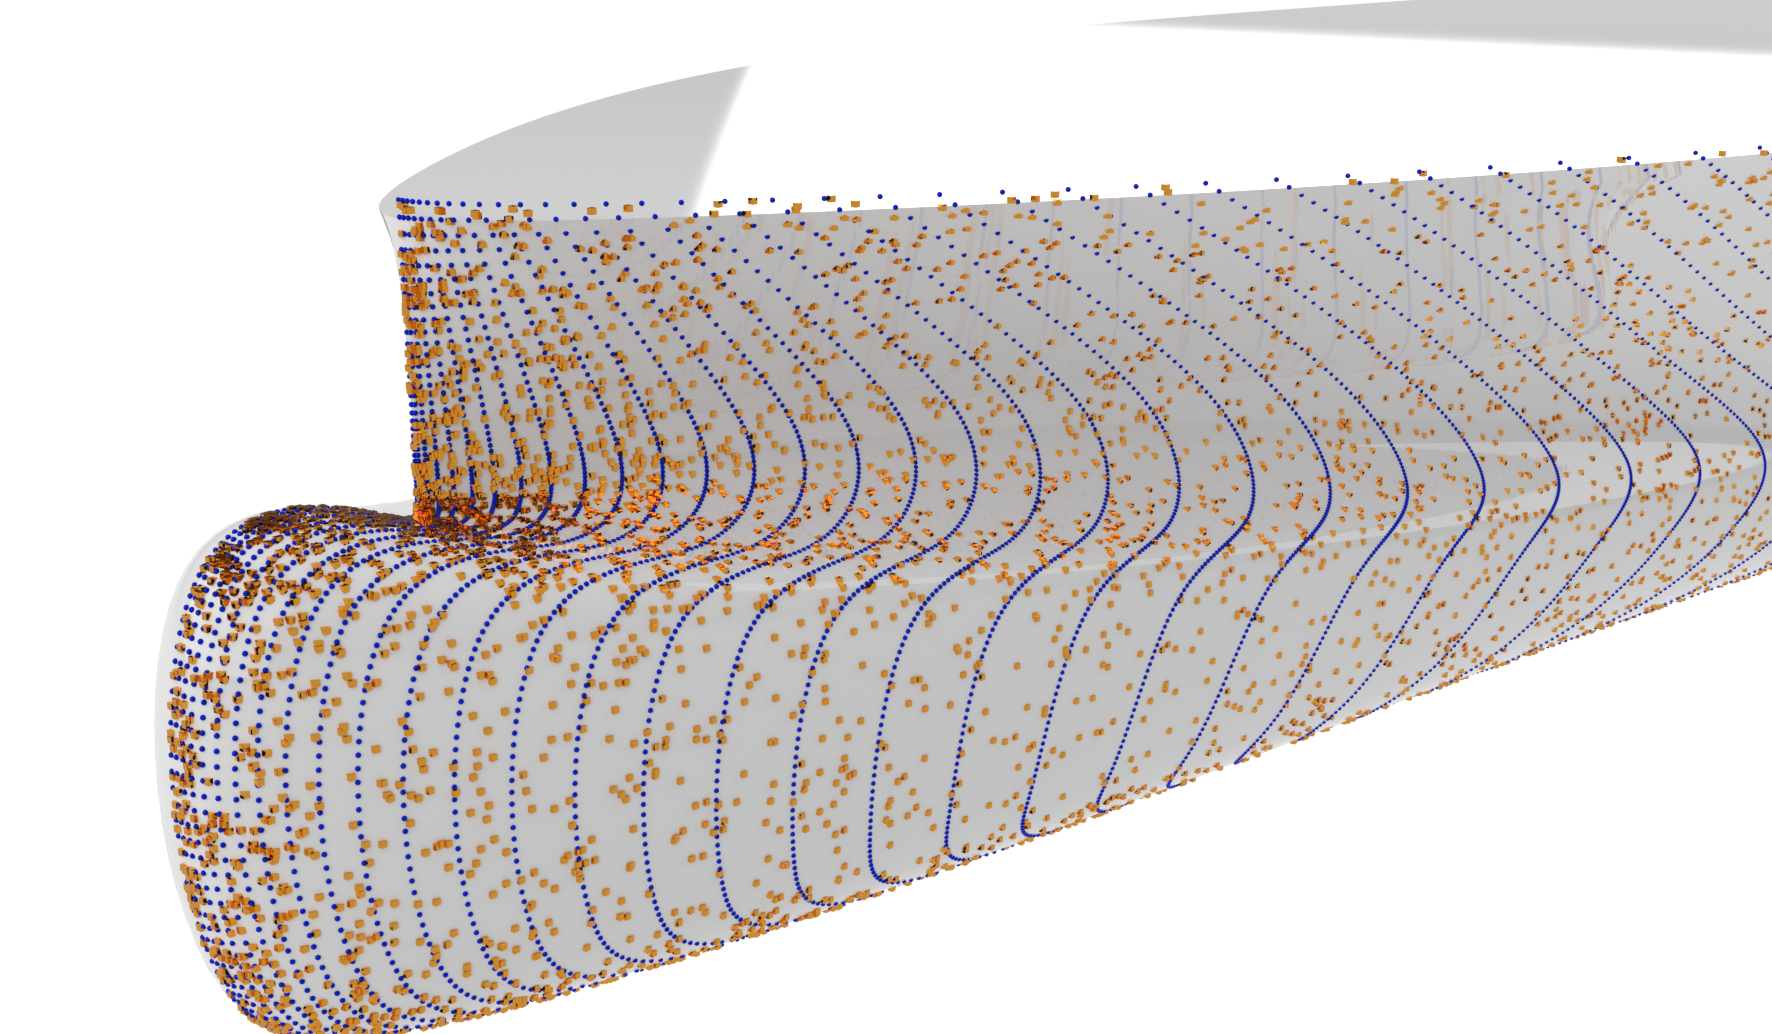
\includegraphics[width = 0.7\linewidth]{figures/test-3-kcssim-random-uniform-render.png}
    \caption{Render of bow-section of KCSsim hull documented in Table \ref{tab:test-3-kcssim-design},
    with two point clouds: a uniformly generated point cloud (blue spheres) and a randomly generated 
    point cloud (bronze cubes)}
    \label{fig:test-3-kcssim-random-uniform-render}
\end{figure}
\begin{figure}[H]
    \centering
    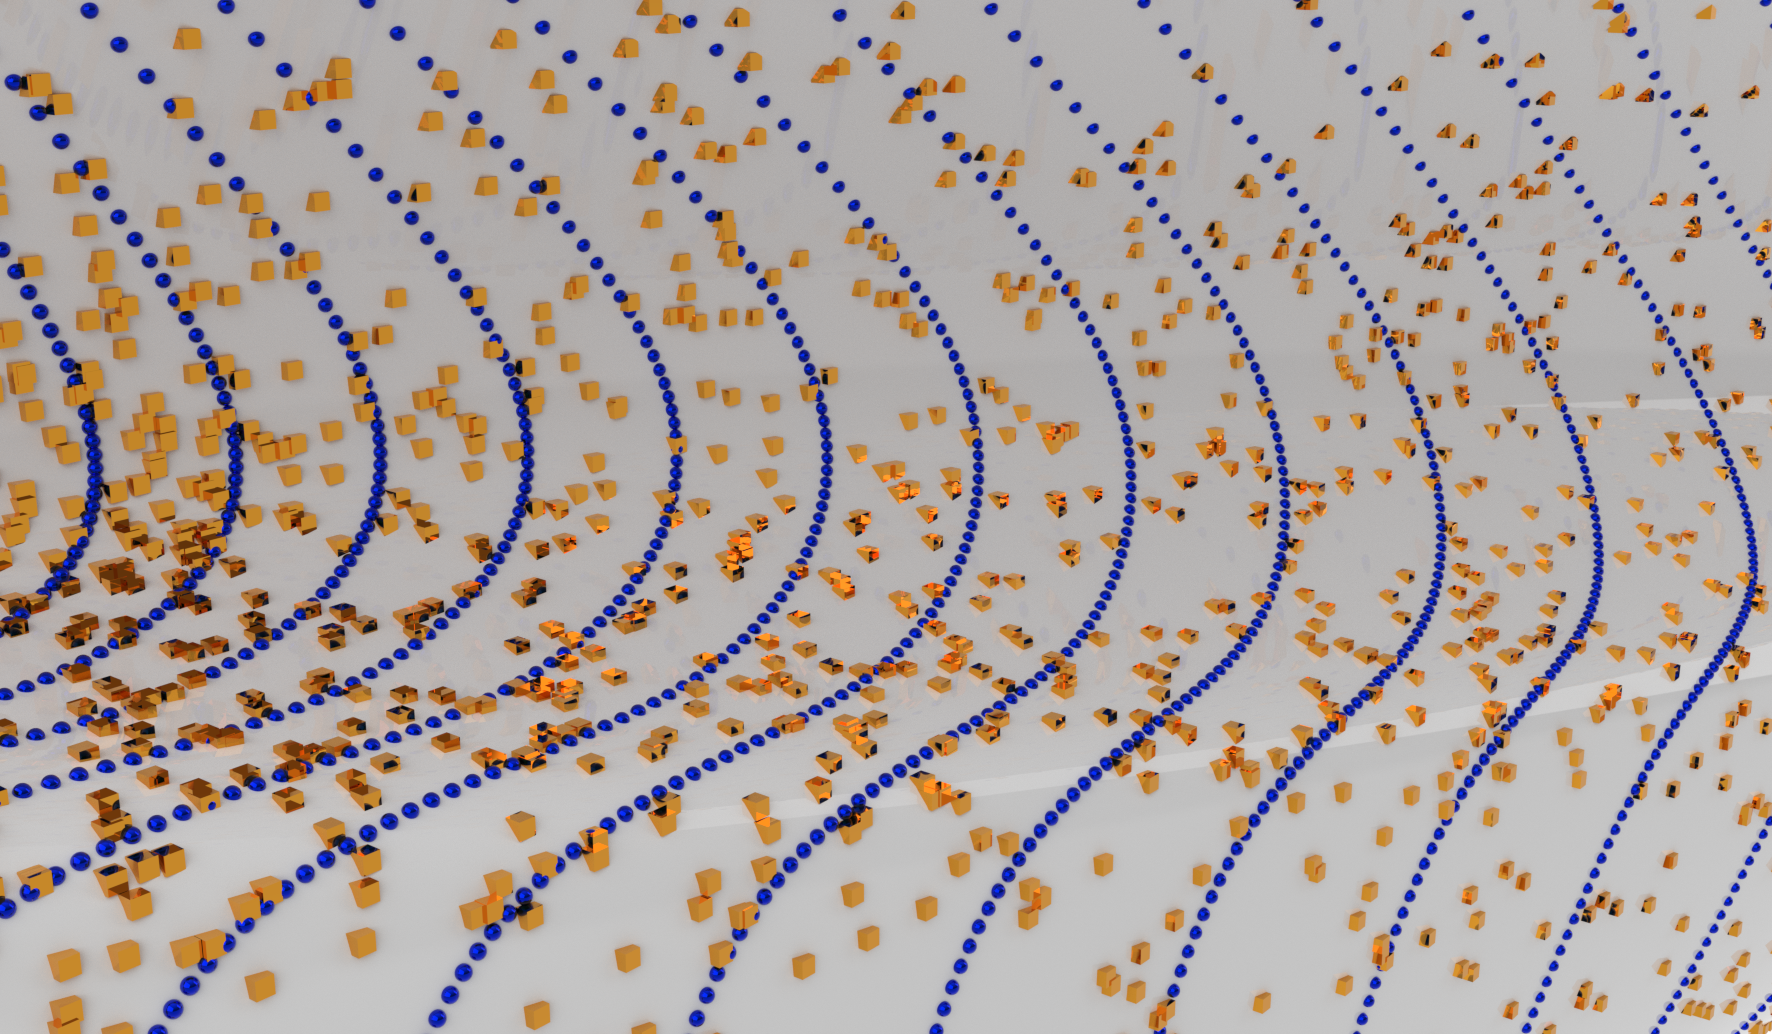
\includegraphics[width = 0.7\linewidth]{figures/test-3-kcssim-random-uniform-render-close-up.png}
    \caption{Close-up render of bow-section of KCSsim hull documented in Table \ref{tab:test-3-kcssim-design},
    with two point clouds: a uniformly generated point cloud (blue spheres) and a randomly generated 
    point cloud (bronze cubes)}
    \label{fig:test-3-kcssim-random-uniform-render-close-up}
\end{figure}

\section{\texttt{test-4.cpp}}

\newpar In this test, the KCSsim modeller is supplemented with a procedure 
to evaluate the derivatives of it's sectional area curve at the boundary
points. Then, the curve it-self is evaluated as in Section \ref{sec:test-3}, and the 
image of the differentials of the curve (tangents) are plotted at the 
boundary points. This experiment is repeated across 15 different instances of the 
parametric modeller, including the one used in Section \ref{sec:test-3}. These
have been documented in Appendix \ref{appendix:test-4-graphics}.

\newpar In order to evaluate the directional derivatives at the bow and the aft, two
point clouds are generated and a 1-point numerical differentiation scheme is used.
These point clouds are configured such that for all models they are sufficiently dense and 
close enough to the bow and the aft. To do this, after generating the point cloud, only ones 
that are a specific distance close to the bow and the aft are used for computing the derivative of 
the sectional area curve. See Figure \ref{fig:test-4-experiment-15-render} for an illustration of 
this procedure.

\begin{figure}[H]
    \centering
    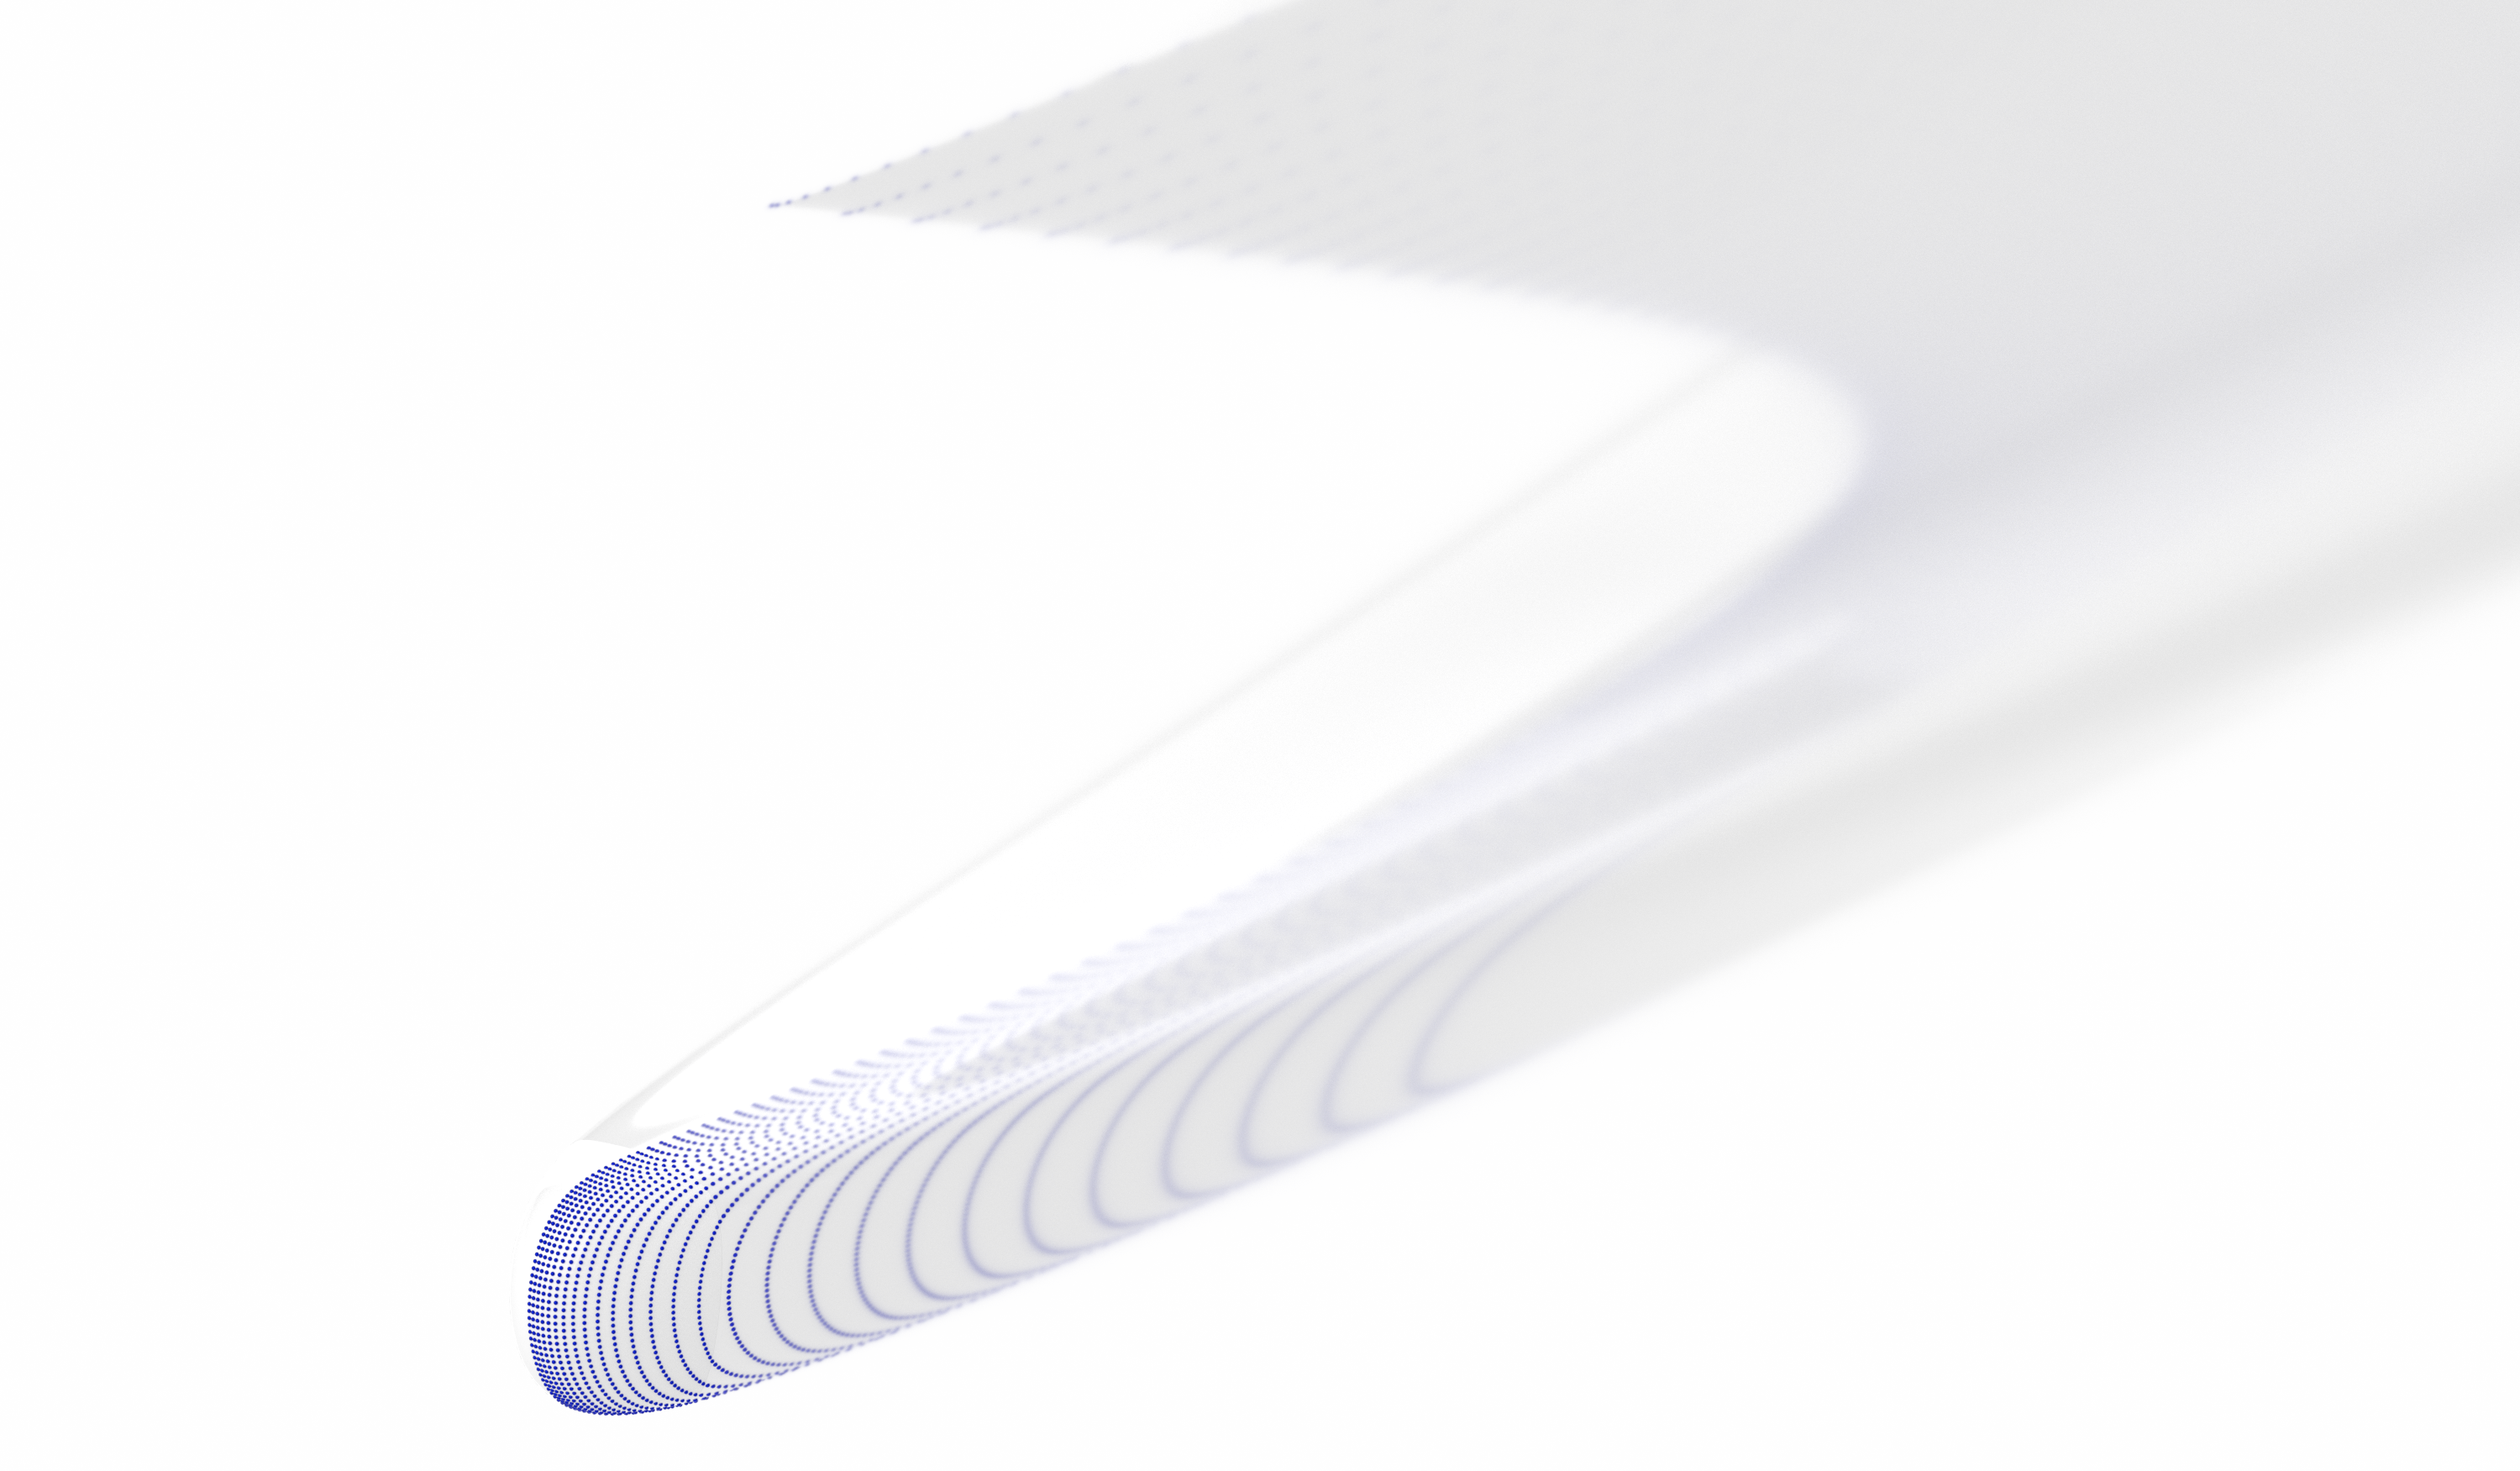
\includegraphics[width=\linewidth]{figures/test-4-experiment-15-render.png}
    \caption{This is the example documented in Table \ref{tab:test-4-15}. The blue points form the 
    bow-generated point cloud, and then the ones behind the frosted screen are discarded. The extra points 
    are necessary because depending on the parametric model, the cloud preimage on the surface's domain is 
    mapped differently onto the surface}
    \label{fig:test-4-experiment-15-render}
\end{figure}

\printbibliography

\appendix

\chapter{\texttt{test-4.cpp}  graphical output}\label{appendix:test-4-graphics}

\begin{table}[H]
    \centering
    \begin{tabular}{|c|c|c|c|c|c|}
        \hline 
        Parameter & Value & Parameter & Value & Parameter & Value\\
        \hline 
        $c_1$ & 1.0 & $c_{11}$ & 0.5 & $c_{21}$ & 1.0 \\
        \hline 
        $c_2$ & 0.8 & $c_{12}$ & 0.5 & $c_{22}$ & 0.0\\
        \hline 
        $c_3$ & 0.8 & $c_{13}$ & 0.5 & $c_{23}$ & 0.5 \\
        \hline 
        $c_4$ & 0.265 & $c_{14}$ & 0.5 & $c_{24}$ & 0.5 \\
        \hline 
        $c_5$ & 0.543 & $c_{15}$ & 0.5 & $c_{25}$ & 0.5 \\
        \hline 
        $c_6$ & 0.0 & $c_{16}$ & 0.05 & $c_{26}$ & 0.5 \\
        \hline 
        $c_7$ & 0.3 & $c_{17}$ & 0.5 & $c_{27}$ & 0.5 \\
        \hline 
        $c_8$ & 0.65 & $c_{18}$ & 0.7 & $c_{28}$ & 0.5 \\
        \hline 
        $c_9$ & 0.7 & $c_{19}$ & 0.8 & $c_{29}$ & 0.5 \\
        \hline 
        $c_{10}$ & 0.5 & $c_{20}$ & 1.0 & - & - \\
        \hline 
    \end{tabular}
    \caption{Design parameters of KCSsim hull with sectional area curve and 
    sectional area curve boundary-derivatives depicted in Figure
    \ref{fig:test-4-sac-1}}
    \label{tab:test-4-1}
\end{table}
\begin{figure}[H]
    \centering
    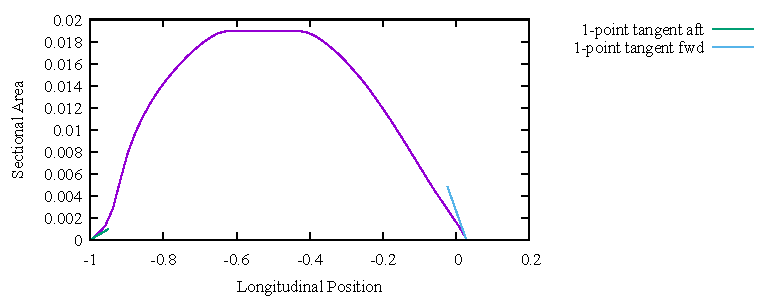
\includegraphics[width = 0.7\linewidth]{figures/test-4-sac-1.pdf}
    \caption{Sectional area curve and boundary approximated derivatives for
    the geometry documented in Table \ref{tab:test-4-1}}
    \label{fig:test-4-sac-1}
\end{figure}
\begin{table}[H]
    \centering
    \begin{tabular}{|c|c|c|c|c|c|}
        \hline 
        Parameter & Value & Parameter & Value & Parameter & Value\\
        \hline 
        $c_1$ & 1.0 & $c_{11}$ & 0.5 & $c_{21}$ & 1.0 \\
        \hline 
        $c_2$ & 0.8 & $c_{12}$ & 0.5 & $c_{22}$ & 0.0\\
        \hline 
        $c_3$ & 0.8 & $c_{13}$ & 0.5 & $c_{23}$ & 0.5 \\
        \hline 
        $c_4$ & 0.265 & $c_{14}$ & 0.5 & $c_{24}$ & 0.5 \\
        \hline 
        $c_5$ & 0.543 & $c_{15}$ & 0.5 & $c_{25}$ & 0.5 \\
        \hline 
        $c_6$ & 0.0 & $c_{16}$ & 0.05 & $c_{26}$ & 0.5 \\
        \hline 
        $c_7$ & 0.3 & $c_{17}$ & 0.5 & $c_{27}$ & 0.5 \\
        \hline 
        $c_8$ & 0.65 & $c_{18}$ & {\color{blue} 1.0} & $c_{28}$ & 0.5 \\
        \hline 
        $c_9$ & 0.7 & $c_{19}$ & 0.8 & $c_{29}$ & 0.5 \\
        \hline 
        $c_{10}$ & 0.5 & $c_{20}$ & 1.0 & - & - \\
        \hline 
    \end{tabular}
    \caption{Design parameters of KCSsim hull with sectional area curve and 
    sectional area curve boundary-derivatives depicted in Figure
    \ref{fig:test-4-sac-2}}
    \label{tab:test-4-2}
\end{table}
\begin{figure}[H]
    \centering
    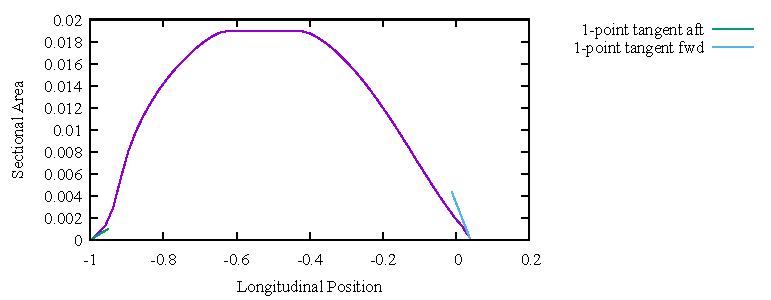
\includegraphics[width = 0.7\linewidth]{figures/test-4-sac-2.pdf}
    \caption{Sectional area curve and boundary approximated derivatives for
    the geometry documented in Table \ref{tab:test-4-2}}
    \label{fig:test-4-sac-2}
\end{figure}
\begin{table}[H]
    \centering
    \begin{tabular}{|c|c|c|c|c|c|}
        \hline 
        Parameter & Value & Parameter & Value & Parameter & Value\\
        \hline 
        $c_1$ & 1.0 & $c_{11}$ & 0.5 & $c_{21}$ & 1.0 \\
        \hline 
        $c_2$ & 0.8 & $c_{12}$ & 0.5 & $c_{22}$ & 0.0\\
        \hline 
        $c_3$ & 0.8 & $c_{13}$ & 0.5 & $c_{23}$ & 0.5 \\
        \hline 
        $c_4$ & 0.265 & $c_{14}$ & 0.5 & $c_{24}$ & 0.5 \\
        \hline 
        $c_5$ & 0.543 & $c_{15}$ & 0.5 & $c_{25}$ & 0.5 \\
        \hline 
        $c_6$ & 0.0 & $c_{16}$ & 0.05 & $c_{26}$ & 0.5 \\
        \hline 
        $c_7$ & 0.3 & $c_{17}$ & 0.5 & $c_{27}$ & 0.5 \\
        \hline 
        $c_8$ & 0.65 & $c_{18}$ & {\color{blue} 0.0} & $c_{28}$ & 0.5 \\
        \hline 
        $c_9$ & 0.7 & $c_{19}$ & 0.8 & $c_{29}$ & 0.5 \\
        \hline 
        $c_{10}$ & 0.5 & $c_{20}$ & 1.0 & - & - \\
        \hline 
    \end{tabular}
    \caption{Design parameters of KCSsim hull with sectional area curve and 
    sectional area curve boundary-derivatives depicted in Figure
    \ref{fig:test-4-sac-3}}
    \label{tab:test-4-3}
\end{table}
\begin{figure}[H]
    \centering
    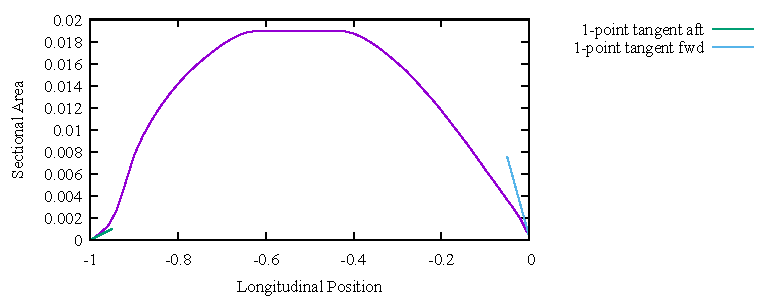
\includegraphics[width = 0.7\linewidth]{figures/test-4-sac-3.pdf}
    \caption{Sectional area curve and boundary approximated derivatives for
    the geometry documented in Table \ref{tab:test-4-3}}
    \label{fig:test-4-sac-3}
\end{figure}
\begin{table}[H]
    \centering
    \begin{tabular}{|c|c|c|c|c|c|}
        \hline 
        Parameter & Value & Parameter & Value & Parameter & Value\\
        \hline 
        $c_1$ & 1.0 & $c_{11}$ & 0.5 & $c_{21}$ & 1.0 \\
        \hline 
        $c_2$ & 0.8 & $c_{12}$ & {\color{blue} 1.0} & $c_{22}$ & 0.0\\
        \hline 
        $c_3$ & 0.8 & $c_{13}$ & 0.5 & $c_{23}$ & 0.5 \\
        \hline 
        $c_4$ & 0.265 & $c_{14}$ & 0.5 & $c_{24}$ & 0.5 \\
        \hline 
        $c_5$ & 0.543 & $c_{15}$ & 0.5 & $c_{25}$ & 0.5 \\
        \hline 
        $c_6$ & 0.0 & $c_{16}$ & 0.05 & $c_{26}$ & 0.5 \\
        \hline 
        $c_7$ & 0.3 & $c_{17}$ & 0.5 & $c_{27}$ & 0.5 \\
        \hline 
        $c_8$ & 0.65 & $c_{18}$ & 0.7 & $c_{28}$ & 0.5 \\
        \hline 
        $c_9$ & 0.7 & $c_{19}$ & 0.8 & $c_{29}$ & 0.5 \\
        \hline 
        $c_{10}$ & 0.5 & $c_{20}$ & 1.0 & - & - \\
        \hline 
    \end{tabular}
    \caption{Design parameters of KCSsim hull with sectional area curve and 
    sectional area curve boundary-derivatives depicted in Figure
    \ref{fig:test-4-sac-4}}
    \label{tab:test-4-4}
\end{table}
\begin{figure}[H]
    \centering
    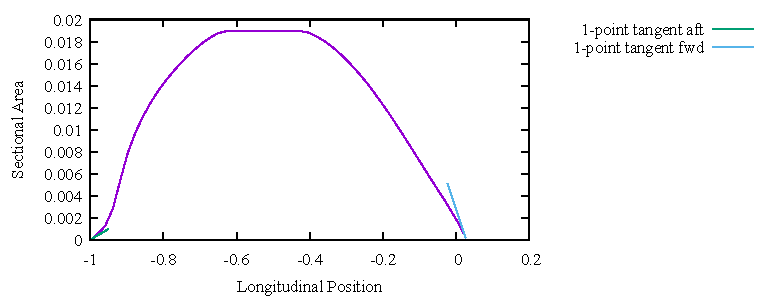
\includegraphics[width = 0.7\linewidth]{figures/test-4-sac-4.pdf}
    \caption{Sectional area curve and boundary approximated derivatives for
    the geometry documented in Table \ref{tab:test-4-4}}
    \label{fig:test-4-sac-4}
\end{figure}
\begin{table}[H]
    \centering
    \begin{tabular}{|c|c|c|c|c|c|}
        \hline 
        Parameter & Value & Parameter & Value & Parameter & Value\\
        \hline 
        $c_1$ & 1.0 & $c_{11}$ & 0.5 & $c_{21}$ & 1.0 \\
        \hline 
        $c_2$ & 0.8 & $c_{12}$ & {\color{blue} 0.0} & $c_{22}$ & 0.0\\
        \hline 
        $c_3$ & 0.8 & $c_{13}$ & 0.5 & $c_{23}$ & 0.5 \\
        \hline 
        $c_4$ & 0.265 & $c_{14}$ & 0.5 & $c_{24}$ & 0.5 \\
        \hline 
        $c_5$ & 0.543 & $c_{15}$ & 0.5 & $c_{25}$ & 0.5 \\
        \hline 
        $c_6$ & 0.0 & $c_{16}$ & 0.05 & $c_{26}$ & 0.5 \\
        \hline 
        $c_7$ & 0.3 & $c_{17}$ & 0.5 & $c_{27}$ & 0.5 \\
        \hline 
        $c_8$ & 0.65 & $c_{18}$ & 0.7 & $c_{28}$ & 0.5 \\
        \hline 
        $c_9$ & 0.7 & $c_{19}$ & 0.8 & $c_{29}$ & 0.5 \\
        \hline 
        $c_{10}$ & 0.5 & $c_{20}$ & 1.0 & - & - \\
        \hline 
    \end{tabular}
    \caption{Design parameters of KCSsim hull with sectional area curve and 
    sectional area curve boundary-derivatives depicted in Figure
    \ref{fig:test-4-sac-5}}
    \label{tab:test-4-5}
\end{table}
\begin{figure}[H]
    \centering
    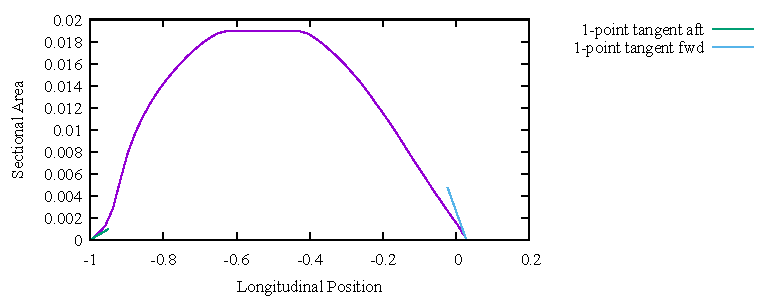
\includegraphics[width = 0.7\linewidth]{figures/test-4-sac-5.pdf}
    \caption{Sectional area curve and boundary approximated derivatives for
    the geometry documented in Table \ref{tab:test-4-5}}
    \label{fig:test-4-sac-5}
\end{figure}
\begin{table}[H]
    \centering
    \begin{tabular}{|c|c|c|c|c|c|}
        \hline 
        Parameter & Value & Parameter & Value & Parameter & Value\\
        \hline 
        $c_1$ & 1.0 & $c_{11}$ & 0.5 & $c_{21}$ & 1.0 \\
        \hline 
        $c_2$ & 0.8 & $c_{12}$ & 0.5 & $c_{22}$ & 0.0\\
        \hline 
        $c_3$ & 0.8 & $c_{13}$ & {\color{blue} 0.0} & $c_{23}$ & 0.5 \\
        \hline 
        $c_4$ & 0.265 & $c_{14}$ & 0.5 & $c_{24}$ & 0.5 \\
        \hline 
        $c_5$ & 0.543 & $c_{15}$ & 0.5 & $c_{25}$ & 0.5 \\
        \hline 
        $c_6$ & 0.0 & $c_{16}$ & 0.05 & $c_{26}$ & 0.5 \\
        \hline 
        $c_7$ & 0.3 & $c_{17}$ & 0.5 & $c_{27}$ & 0.5 \\
        \hline 
        $c_8$ & 0.65 & $c_{18}$ & 0.7 & $c_{28}$ & 0.5 \\
        \hline 
        $c_9$ & 0.7 & $c_{19}$ & 0.8 & $c_{29}$ & 0.5 \\
        \hline 
        $c_{10}$ & 0.5 & $c_{20}$ & 1.0 & - & - \\
        \hline 
    \end{tabular}
    \caption{Design parameters of KCSsim hull with sectional area curve and 
    sectional area curve boundary-derivatives depicted in Figure
    \ref{fig:test-4-sac-6}}
    \label{tab:test-4-6}
\end{table}
\begin{figure}[H]
    \centering
    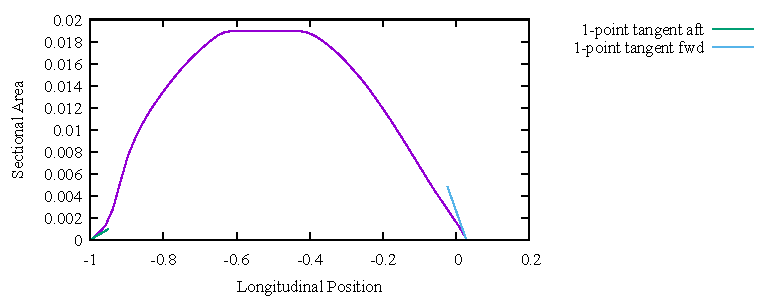
\includegraphics[width = 0.7\linewidth]{figures/test-4-sac-6.pdf}
    \caption{Sectional area curve and boundary approximated derivatives for
    the geometry documented in Table \ref{tab:test-4-6}}
    \label{fig:test-4-sac-6}
\end{figure}
\begin{table}[H]
    \centering
    \begin{tabular}{|c|c|c|c|c|c|}
        \hline 
        Parameter & Value & Parameter & Value & Parameter & Value\\
        \hline 
        $c_1$ & 1.0 & $c_{11}$ & 0.5 & $c_{21}$ & 1.0 \\
        \hline 
        $c_2$ & 0.8 & $c_{12}$ & 0.5 & $c_{22}$ & 0.0\\
        \hline 
        $c_3$ & 0.8 & $c_{13}$ & {\color{blue} 1.0} & $c_{23}$ & 0.5 \\
        \hline 
        $c_4$ & 0.265 & $c_{14}$ & 0.5 & $c_{24}$ & 0.5 \\
        \hline 
        $c_5$ & 0.543 & $c_{15}$ & 0.5 & $c_{25}$ & 0.5 \\
        \hline 
        $c_6$ & 0.0 & $c_{16}$ & 0.05 & $c_{26}$ & 0.5 \\
        \hline 
        $c_7$ & 0.3 & $c_{17}$ & 0.5 & $c_{27}$ & 0.5 \\
        \hline 
        $c_8$ & 0.65 & $c_{18}$ & 0.7 & $c_{28}$ & 0.5 \\
        \hline 
        $c_9$ & 0.7 & $c_{19}$ & 0.8 & $c_{29}$ & 0.5 \\
        \hline 
        $c_{10}$ & 0.5 & $c_{20}$ & 1.0 & - & - \\
        \hline 
    \end{tabular}
    \caption{Design parameters of KCSsim hull with sectional area curve and 
    sectional area curve boundary-derivatives depicted in Figure
    \ref{fig:test-4-sac-7}}
    \label{tab:test-4-7}
\end{table}
\begin{figure}[H]
    \centering
    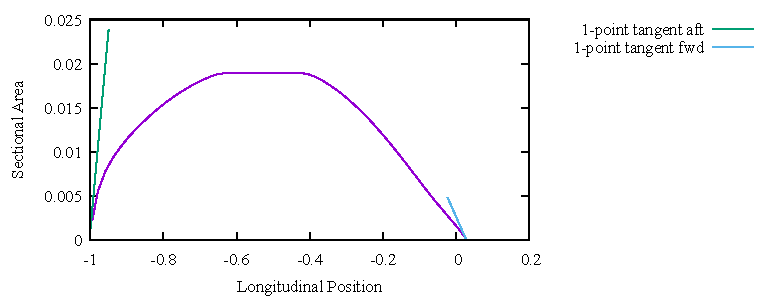
\includegraphics[width = 0.7\linewidth]{figures/test-4-sac-7.pdf}
    \caption{Sectional area curve and boundary approximated derivatives for
    the geometry documented in Table \ref{tab:test-4-7}}
    \label{fig:test-4-sac-7}
\end{figure}
\begin{table}[H]
    \centering
    \begin{tabular}{|c|c|c|c|c|c|}
        \hline 
        Parameter & Value & Parameter & Value & Parameter & Value\\
        \hline 
        $c_1$ & 1.0 & $c_{11}$ & 0.5 & $c_{21}$ & 1.0 \\
        \hline 
        $c_2$ & 0.8 & $c_{12}$ & 0.5 & $c_{22}$ & 0.0\\
        \hline 
        $c_3$ & 0.8 & $c_{13}$ & 0.5 & $c_{23}$ & 0.5 \\
        \hline 
        $c_4$ & 0.265 & $c_{14}$ & 0.5 & $c_{24}$ & 0.5 \\
        \hline 
        $c_5$ & 0.543 & $c_{15}$ & 0.5 & $c_{25}$ & 0.5 \\
        \hline 
        $c_6$ & 0.0 & $c_{16}$ & 0.05 & $c_{26}$ & 0.5 \\
        \hline 
        $c_7$ & 0.3 & $c_{17}$ & 0.5 & $c_{27}$ & {\color{blue} 0.0} \\
        \hline 
        $c_8$ & 0.65 & $c_{18}$ & 0.7 & $c_{28}$ & 0.5 \\
        \hline 
        $c_9$ & 0.7 & $c_{19}$ & 0.8 & $c_{29}$ & 0.5 \\
        \hline 
        $c_{10}$ & 0.5 & $c_{20}$ & 1.0 & - & - \\
        \hline 
    \end{tabular}
    \caption{Design parameters of KCSsim hull with sectional area curve and 
    sectional area curve boundary-derivatives depicted in Figure
    \ref{fig:test-4-sac-8}}
    \label{tab:test-4-8}
\end{table}
\begin{figure}[H]
    \centering
    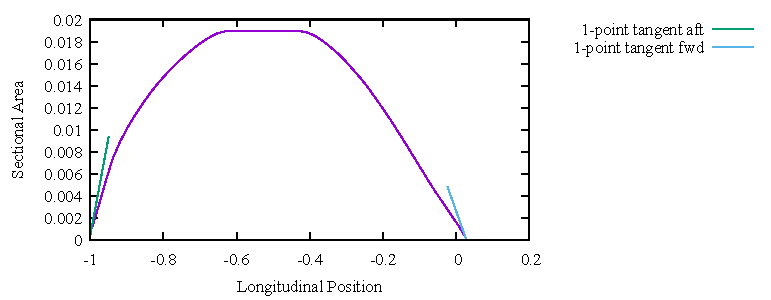
\includegraphics[width = 0.7\linewidth]{figures/test-4-sac-8.pdf}
    \caption{Sectional area curve and boundary approximated derivatives for
    the geometry documented in Table \ref{tab:test-4-8}}
    \label{fig:test-4-sac-8}
\end{figure}
\begin{table}[H]
    \centering
    \begin{tabular}{|c|c|c|c|c|c|}
        \hline 
        Parameter & Value & Parameter & Value & Parameter & Value\\
        \hline 
        $c_1$ & 1.0 & $c_{11}$ & 0.5 & $c_{21}$ & 1.0 \\
        \hline 
        $c_2$ & 0.8 & $c_{12}$ & 0.5 & $c_{22}$ & 0.0\\
        \hline 
        $c_3$ & 0.8 & $c_{13}$ & 0.5 & $c_{23}$ & 0.5 \\
        \hline 
        $c_4$ & 0.265 & $c_{14}$ & 0.5 & $c_{24}$ & 0.5 \\
        \hline 
        $c_5$ & 0.543 & $c_{15}$ & 0.5 & $c_{25}$ & 0.5 \\
        \hline 
        $c_6$ & 0.0 & $c_{16}$ & 0.05 & $c_{26}$ & 0.5 \\
        \hline 
        $c_7$ & 0.3 & $c_{17}$ & 0.5 & $c_{27}$ & {\color{blue} 1.0} \\
        \hline 
        $c_8$ & 0.65 & $c_{18}$ & 0.7 & $c_{28}$ & 0.5 \\
        \hline 
        $c_9$ & 0.7 & $c_{19}$ & 0.8 & $c_{29}$ & 0.5 \\
        \hline 
        $c_{10}$ & 0.5 & $c_{20}$ & 1.0 & - & - \\
        \hline 
    \end{tabular}
    \caption{Design parameters of KCSsim hull with sectional area curve and 
    sectional area curve boundary-derivatives depicted in Figure
    \ref{fig:test-4-sac-9}}
    \label{tab:test-4-9}
\end{table}
\begin{figure}[H]
    \centering
    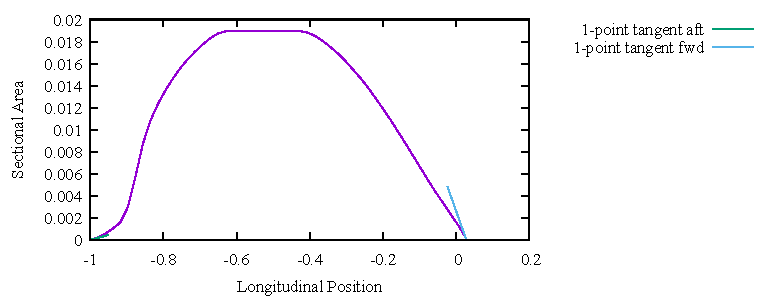
\includegraphics[width = 0.7\linewidth]{figures/test-4-sac-9.pdf}
    \caption{Sectional area curve and boundary approximated derivatives for
    the geometry documented in Table \ref{tab:test-4-9}}
    \label{fig:test-4-sac-9}
\end{figure}
\begin{table}[H]
    \centering
    \begin{tabular}{|c|c|c|c|c|c|}
        \hline 
        Parameter & Value & Parameter & Value & Parameter & Value\\
        \hline 
        $c_1$ & 1.0 & $c_{11}$ & 0.5 & $c_{21}$ & 1.0 \\
        \hline 
        $c_2$ & 0.8 & $c_{12}$ & 0.5 & $c_{22}$ & 0.0\\
        \hline 
        $c_3$ & 0.8 & $c_{13}$ & {\color{blue} 1.0} & $c_{23}$ & 0.5 \\
        \hline 
        $c_4$ & 0.265 & $c_{14}$ & 0.5 & $c_{24}$ & 0.5 \\
        \hline 
        $c_5$ & 0.543 & $c_{15}$ & 0.5 & $c_{25}$ & 0.5 \\
        \hline 
        $c_6$ & 0.0 & $c_{16}$ & 0.05 & $c_{26}$ & 0.5 \\
        \hline 
        $c_7$ & 0.3 & $c_{17}$ & 0.5 & $c_{27}$ & {\color{blue} 0.0} \\
        \hline 
        $c_8$ & 0.65 & $c_{18}$ & 0.7 & $c_{28}$ & 0.5 \\
        \hline 
        $c_9$ & 0.7 & $c_{19}$ & 0.8 & $c_{29}$ & 0.5 \\
        \hline 
        $c_{10}$ & 0.5 & $c_{20}$ & 1.0 & - & - \\
        \hline 
    \end{tabular}
    \caption{Design parameters of KCSsim hull with sectional area curve and 
    sectional area curve boundary-derivatives depicted in Figure
    \ref{fig:test-4-sac-10}}
    \label{tab:test-4-10}
\end{table}
\begin{figure}[H]
    \centering
    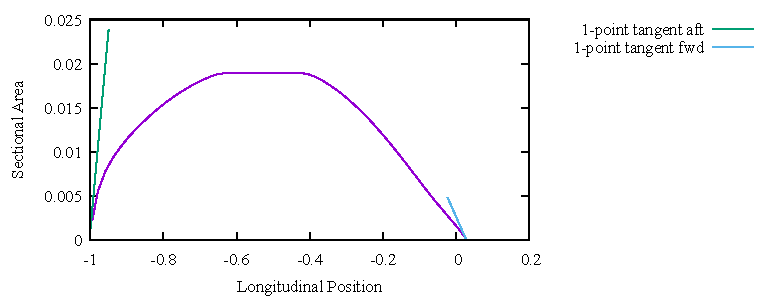
\includegraphics[width = 0.7\linewidth]{figures/test-4-sac-10.pdf}
    \caption{Sectional area curve and boundary approximated derivatives for
    the geometry documented in Table \ref{tab:test-4-10}}
    \label{fig:test-4-sac-10}
\end{figure}
\begin{table}[H]
    \centering
    \begin{tabular}{|c|c|c|c|c|c|}
        \hline 
        Parameter & Value & Parameter & Value & Parameter & Value\\
        \hline 
        $c_1$ & 1.0 & $c_{11}$ & 0.171 & $c_{21}$ & 0.239 \\
        \hline 
        $c_2$ & 0.011 & $c_{12}$ & 0.727 & $c_{22}$ & 0.477\\
        \hline 
        $c_3$ & 0.037 & $c_{13}$ & 0.992 & $c_{23}$ & 0.217 \\
        \hline 
        $c_4$ & 0.165 & $c_{14}$ & 0.597 & $c_{24}$ & 0.482 \\
        \hline 
        $c_5$ & 0.509 & $c_{15}$ & 0.503 & $c_{25}$ & 0.197 \\
        \hline 
        $c_6$ & 0.747 & $c_{16}$ & 0.351 & $c_{26}$ & 0.128 \\
        \hline 
        $c_7$ & 0.343 & $c_{17}$ & 0.397 & $c_{27}$ & 0.789 \\
        \hline 
        $c_8$ & 0.753 & $c_{18}$ & 0.114 & $c_{28}$ & 0.909 \\
        \hline 
        $c_9$ & 0.051 & $c_{19}$ & 0.031 & $c_{29}$ & 0.348 \\
        \hline 
        $c_{10}$ & 0.708 & $c_{20}$ & 0.678 & - & - \\
        \hline 
    \end{tabular}
    \caption{Design parameters of KCSsim hull with sectional area curve and 
    sectional area curve boundary-derivatives depicted in Figure
    \ref{fig:test-4-sac-11}}
    \label{tab:test-4-11}
\end{table}
\begin{figure}[H]
    \centering
    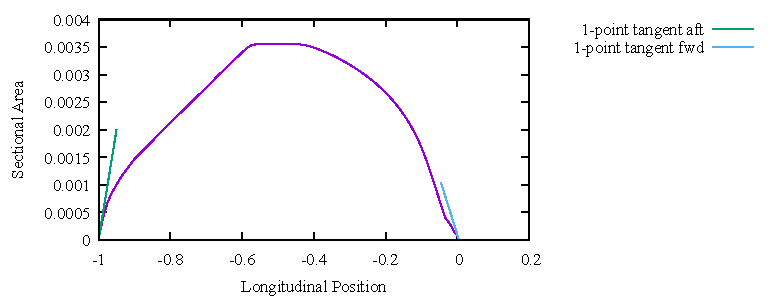
\includegraphics[width = 0.7\linewidth]{figures/test-4-sac-11.pdf}
    \caption{Sectional area curve and boundary approximated derivatives for
    the geometry documented in Table \ref{tab:test-4-11}}
    \label{fig:test-4-sac-11}
\end{figure}
\begin{table}[H]
    \centering
    \begin{tabular}{|c|c|c|c|c|c|}
        \hline 
        Parameter & Value & Parameter & Value & Parameter & Value\\
        \hline 
        $c_1$ & 1.0 & $c_{11}$ & 0.984 & $c_{21}$ & 0.957 \\
        \hline 
        $c_2$ & 0.011 & $c_{12}$ & 0.722 & $c_{22}$ & 0.825\\
        \hline 
        $c_3$ & 0.365 & $c_{13}$ & 0.993 & $c_{23}$ & 0.689 \\
        \hline 
        $c_4$ & 0.710 & $c_{14}$ & 0.272 & $c_{24}$ & 0.940 \\
        \hline 
        $c_5$ & 0.244 & $c_{15}$ & 0.008 & $c_{25}$ & 0.411 \\
        \hline 
        $c_6$ & 0.062 & $c_{16}$ & 0.029 & $c_{26}$ & 0.573 \\
        \hline 
        $c_7$ & 0.463 & $c_{17}$ & 0.926 & $c_{27}$ & 0.126 \\
        \hline 
        $c_8$ & 0.848 & $c_{18}$ & 0.933 & $c_{28}$ & 0.560 \\
        \hline 
        $c_9$ & 0.962 & $c_{19}$ & 0.593 & $c_{29}$ & 0.850 \\
        \hline 
        $c_{10}$ & 0.212 & $c_{20}$ & 0.734 & - & - \\
        \hline 
    \end{tabular}
    \caption{Design parameters of KCSsim hull with sectional area curve and 
    sectional area curve boundary-derivatives depicted in Figure
    \ref{fig:test-4-sac-12}}
    \label{tab:test-4-12}
\end{table}
\begin{figure}[H]
    \centering
    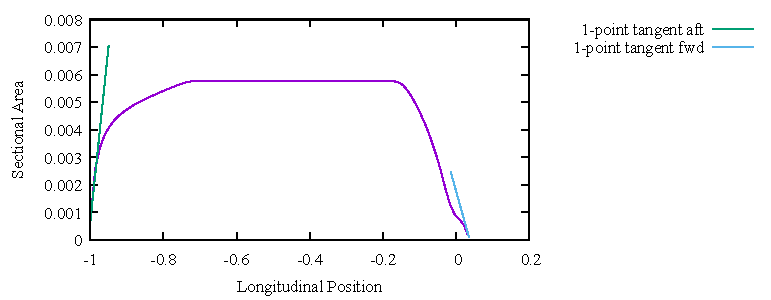
\includegraphics[width = 0.7\linewidth]{figures/test-4-sac-12.pdf}
    \caption{Sectional area curve and boundary approximated derivatives for
    the geometry documented in Table \ref{tab:test-4-12}}
    \label{fig:test-4-sac-12}
\end{figure}
\begin{table}[H]
    \centering
    \begin{tabular}{|c|c|c|c|c|c|}
        \hline 
        Parameter & Value & Parameter & Value & Parameter & Value\\
        \hline 
        $c_1$ & 1.0 & $c_{11}$ & 0.796 & $c_{21}$ & 0.675 \\
        \hline 
        $c_2$ & 0.011 & $c_{12}$ & 0.718 & $c_{22}$ & 0.174\\
        \hline 
        $c_3$ & 0.693 & $c_{13}$ & 0.994 & $c_{23}$ & 0.162 \\
        \hline 
        $c_4$ & 0.255 & $c_{14}$ & 0.948 & $c_{24}$ & 0.398 \\
        \hline 
        $c_5$ & 0.978 & $c_{15}$ & 0.513 & $c_{25}$ & 0.625 \\
        \hline 
        $c_6$ & 0.377 & $c_{16}$ & 0.706 & $c_{26}$ & 0.019 \\
        \hline 
        $c_7$ & 0.583 & $c_{17}$ & 0.455 & $c_{27}$ & 0.464 \\
        \hline 
        $c_8$ & 0.943 & $c_{18}$ & 0.751 & $c_{28}$ & 0.210 \\
        \hline 
        $c_9$ & 0.873 & $c_{19}$ & 0.156 & $c_{29}$ & 0.353 \\
        \hline 
        $c_{10}$ & 0.716 & $c_{20}$ & 0.790 & - & - \\
        \hline 
    \end{tabular}
    \caption{Design parameters of KCSsim hull with sectional area curve and 
    sectional area curve boundary-derivatives depicted in Figure
    \ref{fig:test-4-sac-13}}
    \label{tab:test-4-13}
\end{table}
\begin{figure}[H]
    \centering
    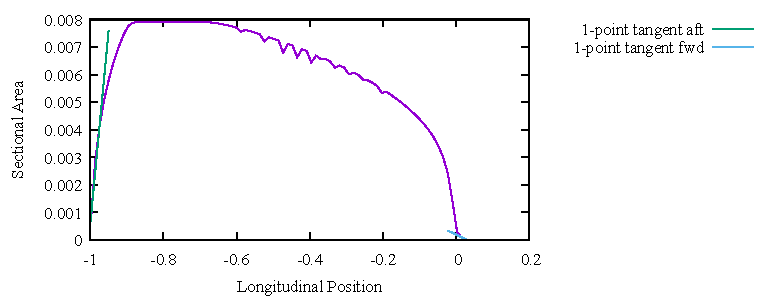
\includegraphics[width = 0.7\linewidth]{figures/test-4-sac-13.pdf}
    \caption{Sectional area curve and boundary approximated derivatives for
    the geometry documented in Table \ref{tab:test-4-13}}
    \label{fig:test-4-sac-13}
\end{figure}
\begin{table}[H]
    \centering
    \begin{tabular}{|c|c|c|c|c|c|}
        \hline 
        Parameter & Value & Parameter & Value & Parameter & Value\\
        \hline 
        $c_1$ & 1.0 & $c_{11}$ & 0.608 & $c_{21}$ & 0.393 \\
        \hline 
        $c_2$ & 0.011 & $c_{12}$ & 0.713 & $c_{22}$ & 0.522\\
        \hline 
        $c_3$ & 0.021 & $c_{13}$ & 0.996 & $c_{23}$ & 0.634 \\
        \hline 
        $c_4$ & 0.800 & $c_{14}$ & 0.624 & $c_{24}$ & 0.857 \\
        \hline 
        $c_5$ & 0.712 & $c_{15}$ & 0.018 & $c_{25}$ & 0.839 \\
        \hline 
        $c_6$ & 0.692 & $c_{16}$ & 0.383 & $c_{26}$ & 0.464 \\
        \hline 
        $c_7$ & 0.702 & $c_{17}$ & 0.984 & $c_{27}$ & 0.801 \\
        \hline 
        $c_8$ & 0.038 & $c_{18}$ & 0.570 & $c_{28}$ & 0.860 \\
        \hline 
        $c_9$ & 0.783 & $c_{19}$ & 0.718 & $c_{29}$ & 0.856 \\
        \hline 
        $c_{10}$ & 0.219 & $c_{20}$ & 0.846 & - & - \\
        \hline 
    \end{tabular}
    \caption{Design parameters of KCSsim hull with sectional area curve and 
    sectional area curve boundary-derivatives depicted in Figure
    \ref{fig:test-4-sac-14}}
    \label{tab:test-4-14}
\end{table}
\begin{figure}[H]
    \centering
    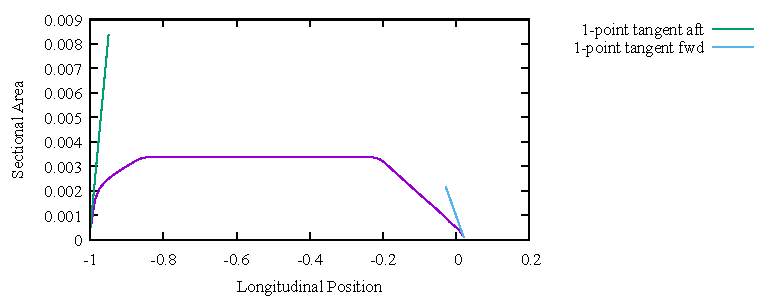
\includegraphics[width = 0.7\linewidth]{figures/test-4-sac-14.pdf}
    \caption{Sectional area curve and boundary approximated derivatives for
    the geometry documented in Table \ref{tab:test-4-14}}
    \label{fig:test-4-sac-14}
\end{figure}
\begin{table}[H]
    \centering
    \begin{tabular}{|c|c|c|c|c|c|}
        \hline 
        Parameter & Value & Parameter & Value & Parameter & Value\\
        \hline 
        $c_1$ & 1.0 & $c_{11}$ & 0.421 & $c_{21}$ & 0.111 \\
        \hline 
        $c_2$ & 0.011 & $c_{12}$ & 0.709 & $c_{22}$ & 0.870\\
        \hline 
        $c_3$ & 0.349 & $c_{13}$ & 0.997 & $c_{23}$ & 0.107 \\
        \hline 
        $c_4$ & 0.345 & $c_{14}$ & 0.299 & $c_{24}$ & 0.315 \\
        \hline 
        $c_5$ & 0.447 & $c_{15}$ & 0.523 & $c_{25}$ & 0.053 \\
        \hline 
        $c_6$ & 0.006 & $c_{16}$ & 0.060 & $c_{26}$ & 0.910 \\
        \hline 
        $c_7$ & 0.822 & $c_{17}$ & 0.513 & $c_{27}$ & 0.139 \\
        \hline 
        $c_8$ & 0.133 & $c_{18}$ & 0.388 & $c_{28}$ & 0.511 \\
        \hline 
        $c_9$ & 0.694 & $c_{19}$ & 0.280 & $c_{29}$ & 0.359 \\
        \hline 
        $c_{10}$ & 0.723 & $c_{20}$ & 0.901 & - & - \\
        \hline 
    \end{tabular}
    \caption{Design parameters of KCSsim hull with sectional area curve and 
    sectional area curve boundary-derivatives depicted in Figure
    \ref{fig:test-4-sac-15}}
    \label{tab:test-4-15}
\end{table}
\begin{figure}[H]
    \centering
    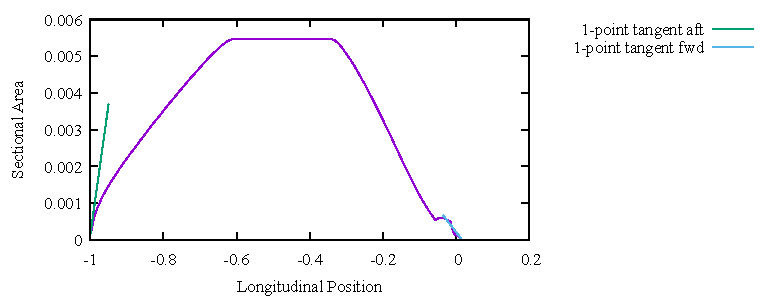
\includegraphics[width = 0.7\linewidth]{figures/test-4-sac-15.pdf}
    \caption{Sectional area curve and boundary approximated derivatives for
    the geometry documented in Table \ref{tab:test-4-15}}
    \label{fig:test-4-sac-15}
\end{figure}
\end{document}